\documentclass[aspectratio=169,xcolor=table]{beamer}

\usetheme{SimpleDarkBlue}
\setbeamertemplate{navigation symbols}{}
\setbeamertemplate{caption}[numbered]

\usepackage[utf8]{inputenc}
\usepackage{tikz}
\usetikzlibrary{shapes,arrows,positioning,fit,backgrounds,mindmap,trees}
\usepackage{listings}
\usepackage{xcolor}
\usepackage{booktabs}
\usepackage{array}
\usepackage{multirow}
\usepackage{enumitem}
\def\labelenumi{\theenumi}
\renewcommand{\labelenumi}{\alph{enumi}.)}
\definecolor{mygreen}{RGB}{28,172,0}
\definecolor{myblue}{RGB}{0,112,192}
\definecolor{myred}{RGB}{192,0,0}

\title{Architektura monolityczna i mikroserwisowa: analiza porównawcza i praktyczne zastosowania}
\subtitle{Podejścia architektoniczne w projektowaniu współczesnych systemów informatycznych\\Projektowanie Systemów Rozproszonych}
\author{mgr inż. Jakub Woźniak}
\institute[PUT]{Zakład Systemów Informatycznych\\Instytut Informatyki Politechniki Poznańskiej}
\date{}

\begin{document}

\begin{frame}
  \titlepage
\end{frame}

\begin{frame}{Plan wykładu}
  \tableofcontents
\end{frame}

\section{Wprowadzenie do architektur systemowych}

\begin{frame}{Ewolucja architektur systemowych}
  \begin{itemize}
    \item Od systemów scentralizowanych do rozproszonych
    \item Wyzwania współczesnych systemów:
      \begin{itemize}
        \item Skalowalność
        \item Odporność na awarie
        \item Szybki rozwój funkcjonalności
        \item Zróżnicowane obciążenie
      \end{itemize}
    \item Dlaczego architektura ma znaczenie:
      \begin{itemize}
        \item Determinuje ograniczenia i możliwości systemu
        \item Wpływa na jakość, wydajność i utrzymywalność
        \item Decyduje o kosztach rozwoju w długim terminie
      \end{itemize}
  \end{itemize}
\end{frame}

\section{Architektura monolityczna}

\begin{frame}{Architektura monolityczna - definicja}
  \begin{block}{Definicja formalna}
    System zbudowany jako \textbf{pojedyncza, spójna jednostka}, gdzie wszystkie komponenty (frontend, backend, baza danych) są ściśle ze sobą zintegrowane i współdzielą ten sam kod oraz zasoby.
  \end{block}
  
  \begin{center}
    \begin{tikzpicture}
      \draw [fill=blue!20, rounded corners] (0,0) rectangle (10,5);
      \node at (5,4.5) {\large\textbf{Aplikacja monolityczna}};
      
      \draw [fill=green!20] (0.5,0.5) rectangle (3.5,2);
      \node at (2,1.25) {Frontend};
      
      \draw [fill=red!20] (0.5,2.5) rectangle (3.5,4);
      \node at (2,3.25) {Backend};
      
      \draw [fill=yellow!20] (4,0.5) rectangle (9.5,2);
      \node at (6.75,1.25) {Warstwa biznesowa};
      
      \draw [fill=orange!20] (4,2.5) rectangle (9.5,4);
      \node at (6.75,3.25) {Dostęp do danych};
      
      \draw[<->, thick] (2,2.25) -- (2,2.25);
      \draw[<->, thick] (3.5,1.25) -- (4,1.25);
      \draw[<->, thick] (3.5,3.25) -- (4,3.25);
      \draw[<->, thick] (6.75,2.25) -- (6.75,2.25);
    \end{tikzpicture}
  \end{center}
\end{frame}

\begin{frame}{Charakterystyka architektury monolitycznej}
  \begin{columns}
    \column{0.5\textwidth}
    \textbf{Cechy strukturalne:}
    \begin{itemize}
      \item Jeden kod bazowy
      \item Jedna baza danych
      \item Jeden proces/kontener
      \item Wspólna kompilacja i wdrożenie
      \item Silne zależności między modułami
    \end{itemize}
    
    \column{0.5\textwidth}
    \textbf{Właściwości operacyjne:}
    \begin{itemize}
      \item Proste wdrażanie (jeden plik)
      \item Scentralizowane zarządzanie
      \item Synchroniczne interakcje między komponentami
      \item Jednolity stack technologiczny
      \item Globalne skalowanie systemu
    \end{itemize}
  \end{columns}
\end{frame}

\begin{frame}{Przykłady monolitów z realnego świata}
  \begin{itemize}
    \item \textbf{Amazon (przed 2001):}
      \begin{itemize}
        \item Jednolity system obsługujący całą logikę e-commerce
        \item Trudności w skalowaniu wraz ze wzrostem ruchu
        \item Problemy z wprowadzaniem zmian przy rosnącej bazie kodu
      \end{itemize}
    \item \textbf{Netflix (wczesna wersja):}
      \begin{itemize}
        \item Monolityczna aplikacja do zarządzania streamingiem
        \item Awarie bazodanowe przy wzroście ruchu
        \item Ograniczona elastyczność technologiczna
      \end{itemize}
    \item \textbf{Uber (początkowo):}
      \begin{itemize}
        \item Jeden kod odpowiedzialny za łączenie kierowców z pasażerami
        \item Ten sam system obsługiwał płatności, zarządzanie przejazdami
        \item Rosnące problemy z utrzymaniem i rozwojem
      \end{itemize}
  \end{itemize}
\end{frame}

\begin{frame}{Cykl życia monolitu}
  \begin{center}
    \begin{tikzpicture}
      \tikzstyle{phase} = [circle, draw, fill=blue!20, minimum size=2cm]
      
      \node[phase] (p1) at (0,0) {Startujący projekt};
      \node[phase] (p2) at (4,0) {Rosnący monolit};
      \node[phase] (p3) at (8,0) {Problematyczny monolit};
      \node[phase] (p4) at (4,-4) {Rozproszony system};
      
      \draw[->, thick] (p1) -- (p2) node[midway, above] {Rozwój};
      \draw[->, thick] (p2) -- (p3) node[midway, above] {Komplikacja};
      \draw[->, thick, dashed] (p3) -- (p4) node[midway, right] {Dekompozycja};
      \draw[->, thick, dashed] (p4) -- (p1) node[midway, left] {Nowe projekty};
    \end{tikzpicture}
  \end{center}
  
  \begin{itemize}
    \item \textbf{Startujący projekt:} Szybki rozwój, łatwość wprowadzania zmian
    \item \textbf{Rosnący monolit:} Narastająca złożoność, spowolnienie rozwoju
    \item \textbf{Problematyczny monolit:} Trudności ze skalowaniem, konflikty deweloperskie
    \item \textbf{Rozproszony system:} Dekompozycja na mniejsze, niezależne części
  \end{itemize}
\end{frame}

\section{Architektura mikroserwisowa}

\begin{frame}{Architektura mikroserwisowa - definicja}
  \begin{block}{Definicja formalna}
    Zbiór niezależnych, samodzielnych usług komunikujących się przez API, z dedykowanymi bazami danych i możliwością niezależnego skalowania.
  \end{block}
  
  \begin{center}
    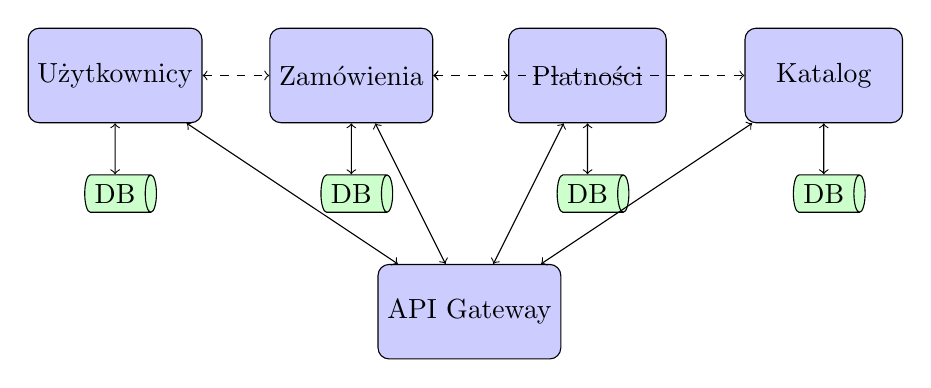
\begin{tikzpicture}
      \tikzstyle{service} = [rectangle, rounded corners, draw, fill=blue!20, minimum width=2cm, minimum height=1.2cm]
      \tikzstyle{db} = [cylinder, draw, shape aspect=0.3, fill=green!20, minimum height=0.8cm]
      
      \node[service] (s1) at (0,4) {Użytkownicy};
      \node[service] (s2) at (3,4) {Zamówienia};
      \node[service] (s3) at (6,4) {Płatności};
      \node[service] (s4) at (9,4) {Katalog};
      
      \node[db] (db1) at (0,2.5) {DB};
      \node[db] (db2) at (3,2.5) {DB};
      \node[db] (db3) at (6,2.5) {DB};
      \node[db] (db4) at (9,2.5) {DB};
      
      \node[service] (api) at (4.5,1) {API Gateway};
      
      \draw[<->, dashed] (s1) -- (s2);
      \draw[<->, dashed] (s2) -- (s3);
      \draw[<->, dashed] (s2) -- (s4);
      
      \draw[<->] (s1) -- (db1);
      \draw[<->] (s2) -- (db2);
      \draw[<->] (s3) -- (db3);
      \draw[<->] (s4) -- (db4);
      
      \draw[<->] (api) -- (s1);
      \draw[<->] (api) -- (s2);
      \draw[<->] (api) -- (s3);
      \draw[<->] (api) -- (s4);
    \end{tikzpicture}
  \end{center}
\end{frame}

\begin{frame}{Charakterystyka architektury mikroserwisowej}
  \begin{columns}
    \column{0.5\textwidth}
    \textbf{Cechy strukturalne:}
    \begin{itemize}
      \item Wiele niezależnych aplikacji
      \item Dedykowane bazy danych
      \item Luźne powiązania (loose coupling)
      \item Autonomia technologiczna
      \item Izolacja awarii (failure isolation)
    \end{itemize}
    
    \column{0.5\textwidth}
    \textbf{Właściwości operacyjne:}
    \begin{itemize}
      \item Niezależne wdrażanie usług
      \item Selektywne skalowanie
      \item Równoległy rozwój przez różne zespoły
      \item Komunikacja przez API (REST, gRPC, etc.)
      \item Rozproszony monitoring i logowanie
    \end{itemize}
  \end{columns}
\end{frame}

\begin{frame}{Przykłady mikroserwisów z realnego świata}
  \begin{itemize}
    \item \textbf{Amazon:}
      \begin{itemize}
        \item Ponad 1000 mikroserwisów po migracji w 2001 roku
        \item Dedykowane usługi dla koszyka, rekomendacji, płatności, wysyłki
        \item Każda strona produktu powstaje z kompozycji wielu usług
      \end{itemize}
    \item \textbf{Netflix:}
      \begin{itemize}
        \item Ponad 700 mikroserwisów w produkcji
        \item Usługi do zarządzania treścią, personalizacji, transkodowania wideo
        \item Architektura oparta na AWS z zaawansowaną instrumentacją
      \end{itemize}
    \item \textbf{Uber:}
      \begin{itemize}
        \item Ponad 500 niezależnych usług
        \item Usługi do zarządzania kierowcami, wyceny przejazdów, notyfikacji
        \item Wykorzystanie mikroserwisów do obsługi usług w różnych regionach
      \end{itemize}
  \end{itemize}
\end{frame}

\begin{frame}{Wzorce komunikacji w mikroserwisach}
  \begin{center}
    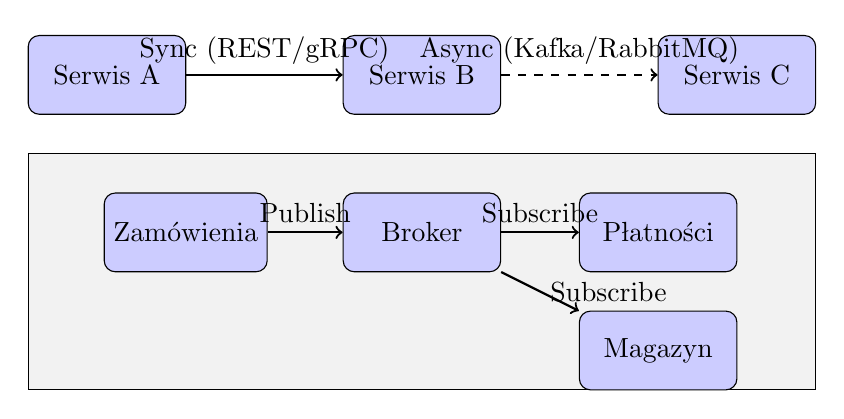
\begin{tikzpicture}
      \tikzstyle{service} = [rectangle, rounded corners, draw, fill=blue!20, minimum width=2cm, minimum height=1cm]
      
      \node[service] (s1) at (0,0) {Serwis A};
      \node[service] (s2) at (4,0) {Serwis B};
      \node[service] (s3) at (8,0) {Serwis C};
      
      \draw[->, thick] (s1) -- (s2) node[midway, above] {Sync (REST/gRPC)};
      \draw[->, thick, dashed] (s2) -- (s3) node[midway, above] {Async (Kafka/RabbitMQ)};
      
      \node[rectangle, draw, fill=gray!10, minimum width=10cm, minimum height=3cm] at (4,-2.5) {};
      
      \node[service] (b1) at (1,-2) {Zamówienia};
      \node[service] (b2) at (4,-2) {Broker};
      \node[service] (b3) at (7,-2) {Płatności};
      \node[service] (b4) at (7,-3.5) {Magazyn};
      
      \draw[->, thick] (b1) -- (b2) node[midway, above] {Publish};
      \draw[->, thick] (b2) -- (b3) node[midway, above] {Subscribe};
      \draw[->, thick] (b2) -- (b4) node[midway, right] {Subscribe};
    \end{tikzpicture}
  \end{center}
  
  \begin{itemize}
    \item \textbf{Synchroniczna:} bezpośrednia odpowiedź, blokująca, REST/gRPC
    \item \textbf{Asynchroniczna:} kolejki wiadomości, event-driven, pub/sub
    \item \textbf{Hybryda:} selektywne użycie obu wzorców zależnie od wymagań
  \end{itemize}
\end{frame}

\section{Porównanie architektur}

\begin{frame}{Szczegółowe porównanie architektur}
  \begin{table}
    \footnotesize
    \begin{tabular}{>{\raggedright\arraybackslash}p{2.8cm}|>{\raggedright\arraybackslash}p{3.8cm}|>{\raggedright\arraybackslash}p{3.8cm}}
      \toprule
      \textbf{Aspekt} & \textbf{Monolit} & \textbf{Mikroserwisy} \\
      \midrule
      \textbf{Rozwój i utrzymanie} & \begin{itemize}[leftmargin=*]
        \item Jeden kod źródłowy
        \item Prostsze debugowanie
        \item Trudna współpraca większych zespołów
      \end{itemize} & \begin{itemize}[leftmargin=*]
        \item Niezależne zespoły na usługach
        \item Większa złożoność całościowa
        \item Równoległy rozwój funkcjonalności
      \end{itemize} \\
      \midrule
      \textbf{Skalowalność} & \begin{itemize}[leftmargin=*]
        \item Skalowanie całości systemu
        \item Nieefektywne przy nierównym obciążeniu
        \item Prostsze mechanizmy
      \end{itemize} & \begin{itemize}[leftmargin=*]
        \item Niezależne skalowanie usług
        \item Optymalizacja zasobów
        \item Złożone strategie skalowania
      \end{itemize} \\
      \bottomrule
    \end{tabular}
  \end{table}
\end{frame}

\begin{frame}{Porównanie architektur (kontynuacja)}
  \begin{table}
    \footnotesize
    \begin{tabular}{>{\raggedright\arraybackslash}p{2.8cm}|>{\raggedright\arraybackslash}p{3.8cm}|>{\raggedright\arraybackslash}p{3.8cm}}
      \toprule
      \textbf{Aspekt} & \textbf{Monolit} & \textbf{Mikroserwisy} \\
      \midrule
      \textbf{Wydajność} & \begin{itemize}[leftmargin=*]
        \item Szybsza komunikacja wewnętrzna
        \item Brak narzutu sieciowego
        \item Mniejsze opóźnienia
      \end{itemize} & \begin{itemize}[leftmargin=*]
        \item Opóźnienia sieciowe
        \item Narzut serializacji/deserializacji
        \item Wyzwania z komunikacją
       \end{itemize} \\
      \midrule
      \textbf{Elastyczność technologiczna} & \begin{itemize}[leftmargin=*]
        \item Ograniczona do jednego stosu
        \item Trudniejsza migracja całości
        \item Spójne biblioteki i narzędzia
      \end{itemize} & \begin{itemize}[leftmargin=*]
        \item Różne języki/frameworki per usługa
        \item Heterogeniczne bazy danych
        \item Łatwiejsza adopcja nowych technologii
      \end{itemize} \\
      \bottomrule
    \end{tabular}
  \end{table}
\end{frame}


\begin{frame}{Porównanie architektur (kontynuacja)}
  \begin{table}
    \footnotesize
    \begin{tabular}{>{\raggedright\arraybackslash}p{2.8cm}|>{\raggedright\arraybackslash}p{3.8cm}|>{\raggedright\arraybackslash}p{3.8cm}}
      \toprule
      \textbf{Aspekt} & \textbf{Monolit} & \textbf{Mikroserwisy} \\
      
      \midrule
      \textbf{Koszty} & \begin{itemize}[leftmargin=*]
        \item Niższe koszty infrastruktury
        \item Mniejsze wymagania operacyjne
        \item Prostsze zarządzanie
      \end{itemize} & \begin{itemize}[leftmargin=*]
        \item Wyższe koszty infrastruktury
        \item Potrzeba zespołu DevOps
        \item Większe nakłady na monitoring
      \end{itemize} \\
      \midrule
      \textbf{Odporność na awarie} & \begin{itemize}[leftmargin=*]
        \item Awaria jednej części wpływa na całość
        \item Prostsze mechanizmy odzyskiwania
        \item Single point of failure
      \end{itemize} & \begin{itemize}[leftmargin=*]
        \item Izolacja awarii pojedynczych usług
        \item Złożona obsługa błędów
        \item Graceful degradation
      \end{itemize} \\
      \bottomrule
    \end{tabular}
  \end{table}
\end{frame}

\begin{frame}{Wizualne porównanie architektury - wzorzec wdrożenia}
  \begin{center}
    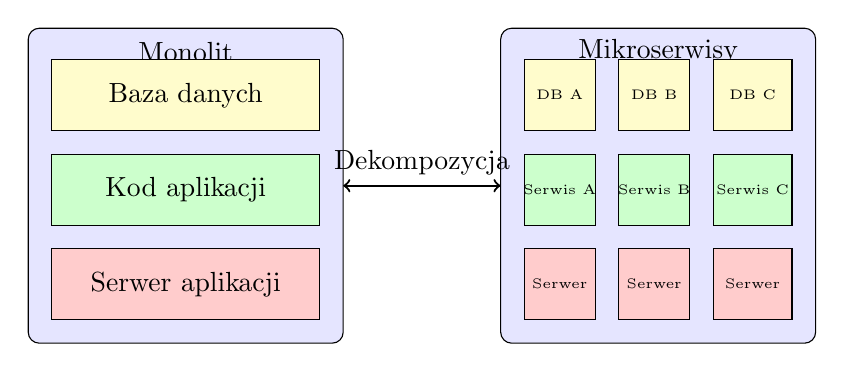
\begin{tikzpicture}
      % Monolit
      \begin{scope}[local bounding box=mono]
        \draw [fill=blue!10, rounded corners] (0,0) rectangle (4,4);
        \node at (2,3.7) {Monolit};
        
        \draw [fill=red!20] (0.3,0.3) rectangle (3.7,1.2);
        \node at (2,0.75) {Serwer aplikacji};
        
        \draw [fill=green!20] (0.3,1.5) rectangle (3.7,2.4);
        \node at (2,1.95) {Kod aplikacji};
        
        \draw [fill=yellow!20] (0.3,2.7) rectangle (3.7,3.6);
        \node at (2,3.15) {Baza danych};
      \end{scope}
      
      % Mikroserwisy
      \begin{scope}[xshift=6cm, local bounding box=micro]
        \draw [fill=blue!10, rounded corners] (0,0) rectangle (4,4);
        \node at (2,3.7) {Mikroserwisy};
        
        \draw [fill=red!20] (0.3,0.3) rectangle (1.2,1.2);
        \node at (0.75,0.75) {\tiny Serwer};
        
        \draw [fill=green!20] (0.3,1.5) rectangle (1.2,2.4);
        \node at (0.75,1.95) {\tiny Serwis A};
        
        \draw [fill=yellow!20] (0.3,2.7) rectangle (1.2,3.6);
        \node at (0.75,3.15) {\tiny DB A};
        
        \draw [fill=red!20] (1.5,0.3) rectangle (2.4,1.2);
        \node at (1.95,0.75) {\tiny Serwer};
        
        \draw [fill=green!20] (1.5,1.5) rectangle (2.4,2.4);
        \node at (1.95,1.95) {\tiny Serwis B};
        
        \draw [fill=yellow!20] (1.5,2.7) rectangle (2.4,3.6);
        \node at (1.95,3.15) {\tiny DB B};
        
        \draw [fill=red!20] (2.7,0.3) rectangle (3.7,1.2);
        \node at (3.2,0.75) {\tiny Serwer};
        
        \draw [fill=green!20] (2.7,1.5) rectangle (3.7,2.4);
        \node at (3.2,1.95) {\tiny Serwis C};
        
        \draw [fill=yellow!20] (2.7,2.7) rectangle (3.7,3.6);
        \node at (3.2,3.15) {\tiny DB C};
      \end{scope}
      
      % Strzałki
      \draw[<->, thick] (mono.east) -- (micro.west) node[midway, above] {Dekompozycja};
    \end{tikzpicture}
  \end{center}
\end{frame}

\section{Szczegółowa analiza mikroserwisów}

\begin{frame}{Zalety architektury mikroserwisowej}
  \begin{columns}
    \column{0.5\textwidth}
    \begin{enumerate}
      \item \textbf{Skalowalność}
        \begin{itemize}
          \item Indywidualne skalowanie usług
          \item Optymalny przydział zasobów
          \item Możliwość skalowania w poziomie
          \item Przykład: Amazon zwiększa moc dla usługi płatności w Black Friday
        \end{itemize}
      
      \item \textbf{Izolacja błędów}
        \begin{itemize}
          \item Awaria jednej usługi nie blokuje systemu
          \item Circuit breaker pattern
          \item Przykład: Netflix Hystrix dla obsługi awarii
        \end{itemize}
    \end{enumerate}
    
    \column{0.5\textwidth}
    \begin{enumerate}\setcounter{enumi}{2}
      \item \textbf{Szybsze wdrażanie}
        \begin{itemize}
          \item Częstsze aktualizacje
          \item Równoległy rozwój przez wiele zespołów
          \item Mniejsze ryzyko zmian
          \item Przykład: Uber wdraża tysiące zmian dziennie
        \end{itemize}
        
      \item \textbf{Elastyczność technologiczna}
        \begin{itemize}
          \item Różne stosy technologiczne
          \item Niezależny wybór języków i baz danych
          \item Przykład: Python dla analityki, Java dla transakcji
        \end{itemize}
    \end{enumerate}
  \end{columns}
\end{frame}

\begin{frame}{Wady architektury mikroserwisowej}
  \begin{columns}
    \column{0.5\textwidth}
    \begin{enumerate}
      \item \textbf{Złożoność zarządzania}
        \begin{itemize}
          \item Potrzeba narzędzi do orkiestracji (Kubernetes)
          \item Wymagania dla monitorowania (Prometheus)
          \item Centralizacja logowania (ELK)
          \item Większa złożoność diagnostyki
        \end{itemize}
      
      \item \textbf{Koszty infrastruktury}
        \begin{itemize}
          \item Zwiększone zapotrzebowanie na zasoby
          \item Każda usługa wymaga osobnych zasobów
          \item Koszty rozproszonych baz danych
        \end{itemize}
    \end{enumerate}
    
    \column{0.5\textwidth}
    \begin{enumerate}\setcounter{enumi}{2}
      \item \textbf{Komunikacja sieciowa}
        \begin{itemize}
          \item Opóźnienia w wywołaniach API
          \item Łańcuchowe zapytania (cascade calls)
          \item Obciążenie sieci wewnętrznej
          \item Narzut na serializację/deserializację
        \end{itemize}
        
      \item \textbf{Spójność danych}
        \begin{itemize}
          \item Brak prostych transakcji
          \item Problemy z danymi rozproszonymi
          \item Złożoność obsługi akcji rozproszonych
        \end{itemize}
    \end{enumerate}
  \end{columns}
\end{frame}

\begin{frame}{Częste pułapki w architekturze mikroserwisowej}
  \begin{enumerate}
    \item \textbf{Niejasne granice usług}
      \begin{itemize}
        \item Tworzenie zbyt drobnych usług (nano-services)
        \item Silnie powiązane usługi (tight coupling)
        \item Rozdzielanie funkcjonalności bez uzasadnienia biznesowego
        \item Przykład: Rozdzielenie uwierzytelnienia i autoryzacji
      \end{itemize}
      
    \item \textbf{Nadmierna inżynieria}
      \begin{itemize}
        \item Przedwczesna mikroserwicyzacja
        \item Implementacja dla prostych systemów bez potrzeby skalowania
        \item Ignorowanie kosztów i złożoności
        \item Przykład: Blog firmowy rozbity na mikroserwisy
      \end{itemize}
    \end{enumerate}
\end{frame}
\begin{frame}{Częste pułapki w architekturze mikroserwisowej}
  \begin{enumerate}\setcounter{enumi}{2}
    \item \textbf{Brak automatyzacji}
      \begin{itemize}
        \item Niewystarczająca infrastruktura CI/CD
        \item Problemy z wersjonowaniem i deployem
        \item Brak zautomatyzowanych testów
      \end{itemize}
      
    \item \textbf{Ignorowanie fundamentów DDD}
      \begin{itemize}
        \item Projektowanie oparte na technologii zamiast domeny
        \item Niespójne modele danych między usługami
        \item Arbitralne granice systemów
      \end{itemize}
  \end{enumerate}
\end{frame}

\section{Domain-Driven Design w mikroserwisach}

\begin{frame}{Fundamenty Domain-Driven Design}
\begin{itemize}
    \item \textbf{Wspólny język (Ubiquitous Language):}
    \begin{itemize}
        \item Jednolity język używany zarówno przez ekspertów domenowych, jak i zespół programistyczny.
        \item Redukuje nieporozumienia i zwiększa spójność w komunikacji.
    \end{itemize}
    \vspace{0.3cm}
    \item \textbf{Konteksty ograniczone (Bounded Contexts):}
    \begin{itemize}
        \item Wyznaczanie granic mikroserwisów w oparciu o naturalne podziały domeny biznesowej.
        \item Każdy kontekst ma własne modele i logikę, co minimalizuje zależności między serwisami.
    \end{itemize}
    \vspace{0.3cm}
\end{itemize}
\end{frame}
\begin{frame}{Fundamenty Domain-Driven Design}
\begin{itemize}
    \item \textbf{Modelowanie strategiczne:}
    \begin{itemize}
        \item Identyfikacja subdomen: core domain (kluczowa domena), supporting domain (wspierająca), generic domain (ogólna).
        \item Pozwala na priorytetyzację obszarów o największym wpływie na biznes.
    \end{itemize}
    \vspace{0.3cm}
    \item \textbf{Modelowanie taktyczne:}
    \begin{itemize}
        \item Projektowanie szczegółowych elementów domeny, takich jak:
        \begin{itemize}
            \item Agregaty
            \item Encje
            \item Serwisy domenowe
        \end{itemize}
        \item Używane do implementacji logiki biznesowej w ramach kontekstu ograniczonego.
    \end{itemize}
\end{itemize}
\end{frame}


\begin{frame}{Kontekst ograniczony (Bounded Context)}
  \begin{center}
    \begin{tikzpicture}
      \tikzstyle{context} = [rectangle, rounded corners, draw, fill=blue!10, minimum width=3.5cm, minimum height=2.5cm]
      \tikzstyle{entity} = [rectangle, draw, fill=green!20, minimum width=2cm, minimum height=0.8cm]
      
      \node[context] (ctx1) at (0,0) {Kontekst Zarządzania Użytkownikami};
      \node[entity] (e1) at (0,0.7) {Użytkownik};
      \node[entity] (e2) at (0,-0.7) {Uprawnienia};
      
      \node[context] (ctx2) at (8,0) {Kontekst Zamówień};
      \node[entity] (e3) at (8,0.7) {Zamówienie};
      \node[entity] (e4) at (8,-0.7) {Klient};
      
      \draw[<->, dashed] (ctx1) -- (ctx2) node[midway, above] {Mapowanie};
      
      \node[below=0.2cm of ctx1] {Użytkownik = osoba z kontem};
      \node[below=0.2cm of ctx2] {Klient = osoba składająca zamówienie};
    \end{tikzpicture}
  \end{center}

  \begin{itemize}
    \item Kontekst ograniczony definiuje granice mikroserwisu w oparciu o domenę biznesową
    \item Każdy kontekst posiada własny model i słownik pojęć
    \item Ten sam termin może mieć różne znaczenie w różnych kontekstach
    \item Implementacja: każdy mikroserwis = jeden bounded context
  \end{itemize}
\end{frame}

\begin{frame}{Mapowanie kontekstów w DDD}
  \begin{table}
    \footnotesize
    \begin{tabular}{>{\raggedright\arraybackslash}p{3cm}|>{\raggedright\arraybackslash}p{7cm}}
      \toprule
      \textbf{Wzorzec mapowania} & \textbf{Charakterystyka} \\
      \midrule
      \textbf{Shared Kernel} & Współdzielona część modelu między kontekstami, wymaga ścisłej koordynacji \\
      \midrule
      \textbf{Customer/Supplier} & Relacja dostawca-odbiorca, zależność jednokierunkowa \\
      \midrule
      \textbf{Conformist} & Jeden kontekst przyjmuje model drugiego bez możliwości wpływu \\
      \midrule
      \textbf{Anticorruption Layer} & Warstwa translacji chroniąca własny model przed zewnętrznym \\
      \midrule
      \textbf{Open Host Service} & Publiczny protokół dostępu do systemu \\
      \midrule
      \textbf{Published Language} & Wspólny format wymiany danych (np. JSON Schema) \\
      \bottomrule
    \end{tabular}
  \end{table}
  
  \begin{itemize}
    \item Mapowanie określa relację między kontekstami/mikroserwisami
    \item Wybór wzorca zależy od relacji zespołów i priorytetów biznesowych
  \end{itemize}
\end{frame}

\begin{frame}{Strategic DDD}
  \begin{center}
    \begin{tikzpicture}
      \tikzstyle{domain} = [rectangle, rounded corners, draw, minimum width=2.5cm, minimum height=1.5cm]
      
      \node[domain, fill=red!20] (core) at (0,2) {Core Domain};
      \node[domain, fill=yellow!20] (supporting) at (6,2) {Supporting Domain};
      \node[domain, fill=green!20] (generic) at (3,0) {Generic Domain};
      
      \draw[->] (core) -- (supporting);
      \draw[->] (core) -- (generic);
      \draw[->] (supporting) -- (generic);
      
      \node[below=0.2cm of core, align=center] {Przewaga konkurencyjna};
      \node[below=0.2cm of supporting, align=center] {Niezbędne, ale nie kluczowe};
      \node[below=0.2cm of generic, align=center] {Rozwiązania standardowe};
    \end{tikzpicture}
  \end{center}

  \begin{itemize}
    \item \textbf{Core Domain:} Najważniejsza część systemu, unikalna wartość biznesowa
      \begin{itemize}
        \item Przykład: Algorytm matchowania Ubera, system rekomendacji Netflixa
        \item Wymaga najlepszych zasobów, in-house development
      \end{itemize}
    \item \textbf{Supporting Domain:} Wspiera Core Domain, ale nie jest unikalna
      \begin{itemize}
        \item Przykład: Profile użytkowników, zarządzanie kontem
      \end{itemize}
    \item \textbf{Generic Domain:} Standardowa funkcjonalność
      \begin{itemize}
        \item Przykład: Uwierzytelnianie, powiadomienia email
        \item Kandydaci do outsourcingu lub gotowych rozwiązań
      \end{itemize}
  \end{itemize}
\end{frame}

\begin{frame}{Tactical DDD}
  \begin{columns}
    \column{0.5\textwidth}
    \begin{center}
      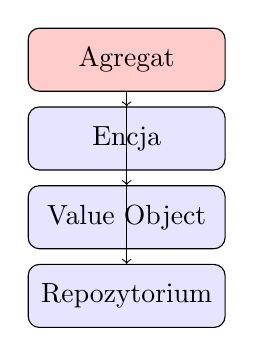
\begin{tikzpicture}
        \tikzstyle{block} = [rectangle, rounded corners, draw, fill=blue!10, minimum width=2.5cm, minimum height=0.8cm]
        
        \node[block, fill=red!20] (agg) at (0,3) {Agregat};
        \node[block] (entity) at (0,2) {Encja};
        \node[block] (vo) at (0,1) {Value Object};
        \node[block] (repo) at (0,0) {Repozytorium};
        
        \draw[->] (agg) -- (entity);
        \draw[->] (entity) -- (vo);
        \draw[->] (agg) -- (repo);
      \end{tikzpicture}
    \end{center}
    
    \column{0.5\textwidth}
    \begin{itemize}
      \item \textbf{Agregat:} Logiczna grupa powiązanych obiektów traktowana jako całość
        \begin{itemize}
          \item Koszyk zakupowy z pozycjami
          \item Zamówienie z adresem dostawy
        \end{itemize}
      \item \textbf{Encja:} Obiekt posiada tożsamość i może zmieniać się w czasie
      \item \textbf{Value Object:} Niemutowalny, bez identyfikatora
      \item \textbf{Repozytorium:} Abstrakcja dostępu do danych
      \item \textbf{Serwis domenowy:} Operacje przekraczające agregaty
    \end{itemize}
  \end{columns}
\end{frame}

\begin{frame}{DDD w praktyce - przykład e-commerce}
  \begin{center}
    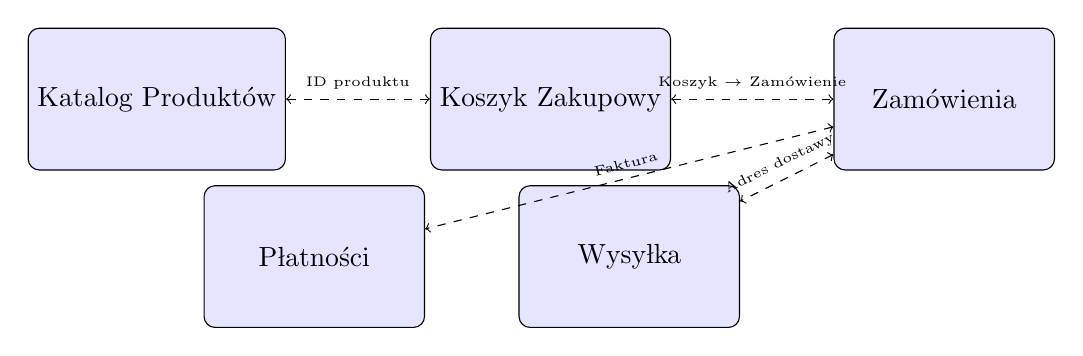
\begin{tikzpicture}
      \tikzstyle{context} = [rectangle, rounded corners, draw, fill=blue!10, minimum width=2.8cm, minimum height=1.8cm]
      
      \node[context] (catalog) at (0,2) {Katalog Produktów};
      \node[context] (cart) at (5,2) {Koszyk Zakupowy};
      \node[context] (order) at (10,2) {Zamówienia};
      \node[context] (payment) at (2,0) {Płatności};
      \node[context] (shipping) at (6,0) {Wysyłka};
      
      \draw[<->, dashed] (catalog) -- (cart) node[midway, above] {\tiny ID produktu};
      \draw[<->, dashed] (cart) -- (order) node[midway, above] {\tiny Koszyk \(\rightarrow\) Zamówienie};
      \draw[<->, dashed] (order) -- (payment) node[midway, above, sloped] {\tiny Faktura};
      \draw[<->, dashed] (order) -- (shipping) node[midway, above, sloped] {\tiny Adres dostawy};
    \end{tikzpicture}
  \end{center}

  \begin{itemize}
    \item Każdy kontekst = osobny mikroserwis z własnym modelem danych
    \item Agregaty:
      \begin{itemize}
        \item \textbf{Katalog:} Produkt (encja) z atrybutami (value objects)
        \item \textbf{Koszyk:} Koszyk (agregat) z pozycjami koszyka (encje)
        \item \textbf{Zamówienia:} Zamówienie (agregat) z pozycjami i statusem
      \end{itemize}
    \item Serwisy domenowe:
      \begin{itemize}
        \item \textbf{Konwersja koszyka na zamówienie, Obsługa procesu płatności}
      \end{itemize}
  \end{itemize}
\end{frame}

\section{Problemy z rozproszonymi transakcjami}

\begin{frame}{Wyzwanie atomowości w systemach rozproszonych}
  \begin{center}
    \begin{tikzpicture}
      \tikzstyle{service} = [rectangle, rounded corners, draw, fill=blue!20, minimum width=2cm, minimum height=1cm]
      
      \node[service] (s1) at (0,0) {Zamówienia};
      \node[service] (s2) at (4,0) {Płatności};
      \node[service] (s3) at (8,0) {Magazyn};
      
      \draw[->, thick] (s1) -- (s2) node[midway, above] {1. Autoryzuj};
      \draw[->, thick] (s2) -- (s3) node[midway, above] {2. Zarezerwuj};
      
      \node[below=0.3cm of s1, align=center] {Status: oczekuje};
      \node[below=0.3cm of s2, align=center] {Płatność: OK};
      \node[below=0.3cm of s3, align=center, text=red] {Brak towaru: błąd!};
      
      \node[below=1.5cm of s2, align=center, text width=10cm] {
        \textbf{Problem:} Brak gwarancji, że wszystkie usługi zatwierdzą swoje operacje.\\
        \textbf{Konsekwencja:} Płatność została zautoryzowana, ale towar niedostępny - konieczność ręcznego wycofania.
      };
    \end{tikzpicture}
  \end{center}
\end{frame}

\begin{frame}{Two-Phase Commit (2PC) - Diagram Sekwencji}
\begin{center}
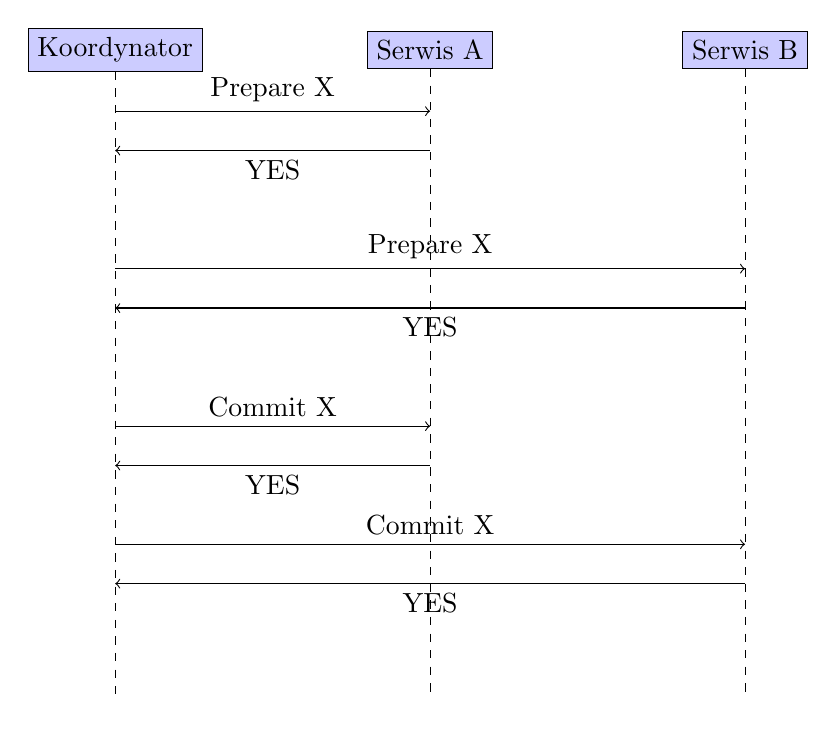
\begin{tikzpicture}[node distance=1.5cm, auto]

  % Define styles for participants
  \tikzstyle{participant} = [rectangle, draw, fill=blue!20, text centered, minimum height=0cm, minimum width=1.5cm]

  % Participants
  \node[participant] (coordinator) at (0,0) {Koordynator};
  \node[participant] (serviceA) at (4,0) {Serwis A};
  \node[participant] (serviceB) at (8,0) {Serwis B};

  % Lifelines
  \draw[dashed] (coordinator.south) -- ++(0,-8) node[below] {};
  \draw[dashed] (serviceA.south) -- ++(0,-8) node[below] {};
  \draw[dashed] (serviceB.south) -- ++(0,-8) node[below] {};

  % Phase 1: Prepare
  \draw[->] (coordinator.south) ++(0,-0.5) -- ++(4,0) node[midway, above] {Prepare X};
  \draw[<-] (coordinator.south) ++(0,-1) -- ++(4,0) node[midway, below] {YES};

  \draw[->] (coordinator.south) ++(0,-2.5) -- ++(8,0) node[midway, above] {Prepare X};
  \draw[<-] (coordinator.south) ++(0,-3) -- ++(8,0) node[midway, below] {YES};

  % Phase 2: Commit
  \draw[->] (coordinator.south) ++(0,-4.5) -- ++(4,0) node[midway, above] {Commit X};
  \draw[<-] (coordinator.south) ++(0,-5) -- ++(4,0) node[midway, below] {YES};

  \draw[->] (coordinator.south) ++(0,-6) -- ++(8,0) node[midway, above] {Commit X};
  \draw[<-] (coordinator.south) ++(0,-6.5) -- ++(8,0) node[midway, below] {YES};

\end{tikzpicture}
\end{center}
\end{frame}

\begin{frame}{Kompromisy spójności - Two-Phase Commit (2PC)}
  \begin{itemize}
    \item \textbf{Zalety:}
      \begin{itemize}
        \item Gwarancja atomowości
        \item Spójność danych
      \end{itemize}
    \item \textbf{Wady:}
      \begin{itemize}
        \item Blokowanie zasobów w fazie przygotowania
        \item Podatność na awarie koordynatora
        \item Problemy z wydajnością
        \item Trudne odzyskiwanie po awarii
      \end{itemize}
  \end{itemize}
\end{frame}

\begin{frame}{Kompromisy spójności - Saga Pattern}
  \begin{center}
    \begin{tikzpicture}
      \tikzstyle{service} = [rectangle, rounded corners, draw, fill=blue!20, minimum width=2cm, minimum height=0.8cm]
      \tikzstyle{compensation} = [rectangle, rounded corners, draw, fill=red!10, minimum width=2cm, minimum height=0.8cm]
      
      \draw [->, thick] (0,0) -- (10,0);
      
      \node[service] (o) at (1,0.7) {Zamówienie};
      \node[service] (p) at (5,0.7) {Płatność};
      \node[service] (s) at (8,0.7) {Magazyn};
      \node[service] (d) at (11,0.7) {Dostawa};
      
      \node[compensation] (cr) at (3,-0.7) {Zwrot};
      \node[compensation] (cg) at (8,-0.7) {Zwrot na stan};
      
      \draw[->] (o) -- (p);
      \draw[->] (p) -- (s);
      \draw[->] (s) -- (d);
      
      \draw[<-, dashed, red] (p) -- (cr);
      \draw[<-, dashed, red] (s) -- (cg);
      
      \draw[->, dashed, red] (s) -- (cr) node[pos=0.3, above, sloped] {błąd};
    \end{tikzpicture}
  \end{center}
  
  \begin{itemize}
    \item \textbf{Definicja:} Sekwencja lokalnych transakcji z mechanizmem kompensacji
    \item \textbf{Zasada działania:}
      \begin{itemize}
        \item Każdy krok to osobna transakcja
        \item Błędy obsługiwane przez transakcje kompensacyjne
        \item Przykład: anulowanie płatności, gdy magazyn zgłasza brak produktu
      \end{itemize}
    \item \textbf{Implementacje:}
      \begin{itemize}
        \item \textbf{Choreografia:} sterowanie przez zdarzenia
        \item \textbf{Orchestracja:} centralny koordynator
      \end{itemize}
  \end{itemize}
\end{frame}

\begin{frame}{Eventual Consistency}
  \begin{center}
    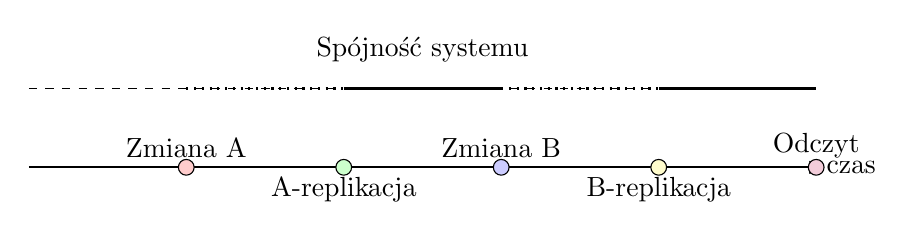
\begin{tikzpicture}
      \draw [->, thick] (0,0) -- (10,0) node[right] {czas};
      
      \filldraw[fill=red!20] (2,0) circle (0.1) node[above] {Zmiana A};
      \filldraw[fill=green!20] (4,0) circle (0.1) node[below] {A-replikacja};
      \filldraw[fill=blue!20] (6,0) circle (0.1) node[above] {Zmiana B};
      \filldraw[fill=yellow!20] (8,0) circle (0.1) node[below] {B-replikacja};
      \filldraw[fill=purple!20] (10,0) circle (0.1) node[above] {Odczyt};
      
      \draw[dashed] (0,1) -- (10,1);
      
      \node at (5,1.5) {Spójność systemu};
      
      \draw[dotted, thick] (2,1) -- (4,1);
      \draw[thick] (4,1) -- (6,1);
      \draw[dotted, thick] (6,1) -- (8,1);
      \draw[thick] (8,1) -- (10,1);
    \end{tikzpicture}
  \end{center}
  
  \begin{itemize}
    \item \textbf{Definicja:} System osiąga spójność danych po pewnym czasie, dopuszczając przejściowe niespójności
    \item \textbf{Zastosowanie:}
      \begin{itemize}
        \item Systemy gdzie szybkość ważniejsza niż absolutna spójność
        \item Mechanizmy synchronizacji oparte o zdarzenia
        \item Przykład: liczba produktów w magazynie, status dostawy
      \end{itemize}
    \item \textbf{Kompromisy:}
      \begin{itemize}
        \item Prostszy model programowania
        \item Lepsza wydajność i dostępność
        \item Konieczność obsługi niespójności przez aplikację
      \end{itemize}
  \end{itemize}
\end{frame}

\begin{frame}{Strategie zarządzania rozproszonymi transakcjami}
  \begin{table}
    \footnotesize
    \begin{tabular}{>{\raggedright\arraybackslash}p{2.8cm}|>{\raggedright\arraybackslash}p{2.8cm}|>{\raggedright\arraybackslash}p{2.8cm}|>{\raggedright\arraybackslash}p{2.8cm}}
      \toprule
      & \textbf{2PC} & \textbf{Saga} & \textbf{Eventual Consistency} \\
      \midrule
      \textbf{Spójność} & Silna & Ostateczna & Ostateczna \\
      \midrule
      \textbf{Wydajność} & Niska & Średnia & Wysoka \\
      \midrule
      \textbf{Złożoność} & Wysoka & Wysoka & Średnia \\
      \midrule
      \textbf{Dostępność} & Niska & Wysoka & Wysoka \\
      \midrule
      \textbf{Najlepsze zastosowania} & Krytyczne operacje finansowe & Procesy biznesowe wieloetapowe & Dane niewymagające natychmiastowej spójności \\
      \midrule
      \textbf{Przykłady} & Przelew z konta na konto & Zamawianie biletów lotniczych & Liczniki wyświetleń, statystyki \\
      \bottomrule
    \end{tabular}
  \end{table}
\end{frame}

\section{Podsumowanie}

\begin{frame}{Wybór odpowiedniej architektury}
  \begin{columns}
    \column{0.5\textwidth}
    \textbf{Kiedy stosować monolity?}
    \begin{itemize}
      \item Małe i średnie projekty
      \item Ograniczone zasoby DevOps
      \item Proste domeny biznesowe
      \item Początkowa faza produktu
      \item Niskie wymagania skalowalności
      \item Brak potrzeby niezależnych wdrożeń
    \end{itemize}
    
    \column{0.5\textwidth}
    \textbf{Kiedy stosować mikroserwisy?}
    \begin{itemize}
      \item Duże, złożone systemy
      \item Wiele niezależnych zespołów
      \item Zróżnicowane wzorce obciążenia
      \item Wysoka skalowalność
      \item Elastyczność technologiczna
      \item Wdrożenia z wysoką częstotliwością
    \end{itemize}
  \end{columns}
\end{frame}

\begin{frame}{Ewolucja zamiast rewolucji}
  \begin{center}
    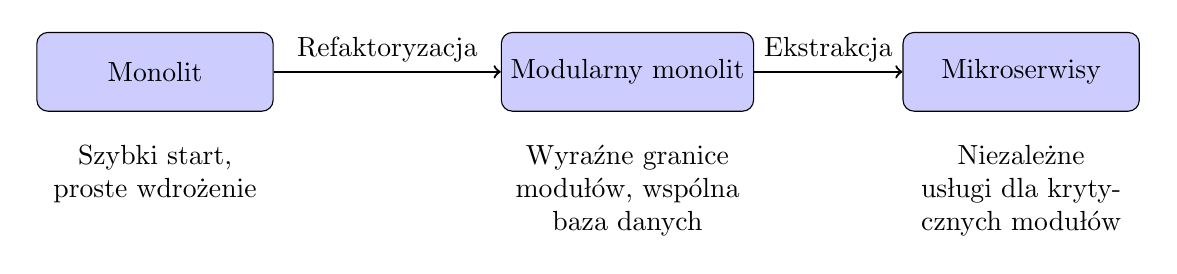
\begin{tikzpicture}
      \tikzstyle{phase} = [rectangle, rounded corners, draw, fill=blue!20, minimum width=3cm, minimum height=1cm]
      
      \node[phase] (p1) at (0,0) {Monolit};
      \node[phase] (p2) at (6,0) {Modularny monolit};
      \node[phase] (p3) at (11,0) {Mikroserwisy};
      
      \draw[->, thick] (p1) -- (p2) node[midway, above] {Refaktoryzacja};
      \draw[->, thick] (p2) -- (p3) node[midway, above] {Ekstrakcja};
      
      \node[below=0.3cm of p1, align=center, text width=3cm] {Szybki start, proste wdrożenie};
      \node[below=0.3cm of p2, align=center, text width=3cm] {Wyraźne granice modułów, wspólna baza danych};
      \node[below=0.3cm of p3, align=center, text width=3cm] {Niezależne usługi dla krytycznych modułów};
    \end{tikzpicture}
  \end{center}
  
  \begin{itemize}
    \item \textbf{Modularny monolit:} Etap pośredni
      \begin{itemize}
        \item Wewnętrzne bounded contexts
        \item Jasno określone granice modułów
        \item Zdefiniowane interfejsy między modułami
        \item Łatwiejsza migracja na mikroserwisy
      \end{itemize}
    \item \textbf{Strategia ekstrakcji:}
      \begin{itemize}
        \item Najpierw wydzielenie najbardziej niezależnych funkcjonalności
        \item Stopniowe zmniejszanie monolitu
        \item Kontrolowane wprowadzanie złożoności
      \end{itemize}
  \end{itemize}
\end{frame}

\begin{frame}{Najważniejsze praktyki i zasady}
  \begin{enumerate}
    \item \textbf{Projektowanie z myślą o domenie biznesowej}
      \begin{itemize}
        \item DDD jako fundament podziału na usługi
        \item Granice usług zgodne z bounded contexts
      \end{itemize}
      
    \item \textbf{Automatyzacja procesów}
      \begin{itemize}
        \item CI/CD jako konieczność dla mikroserwisów
        \item Infrastruktura jako kod (IaC)
        \item Testy automatyczne
      \end{itemize}
      
    \item \textbf{Monitorowanie i obserwowanie}
      \begin{itemize}
        \item Centralne logowanie
        \item Distributed tracing
        \item Metryki wydajności
      \end{itemize}
  \end{enumerate}
\end{frame}     
\begin{frame}{Najważniejsze praktyki i zasady}
  \begin{enumerate}\setcounter{enumi}{3}
    \item \textbf{Przygotowanie na awarie}
      \begin{itemize}
        \item Circuit breakers
        \item Retries with backoff
        \item Fallbacks
        \item Chaos engineering
      \end{itemize}
      
    \item \textbf{Przemyślana strategia danych}
      \begin{itemize}
        \item Świadome kompromisy spójności
        \item Odpowiednie wzorce dla transakcji rozproszonych
        \item Event sourcing jako alternatywa
      \end{itemize}
  \end{enumerate}
\end{frame}

\begin{frame}{Wnioski końcowe}
  \begin{itemize}
    \item Nie ma jednego, optymalnego podejścia dla wszystkich systemów
    \item Mikroserwisy nie są celem, lecz środkiem do osiągnięcia konkretnych wymagań biznesowych
    \item Złożoność rozproszonego systemu zawsze przewyższa złożoność monolitu
    \item Stopniowa ewolucja często jest bezpieczniejsza niż rewolucyjna zmiana
    \item Przemyślany projekt domeny (DDD) jest kluczem do sukcesu obu architektur
    \item Zrozumienie kompromisów i kosztów jest niezbędne dla podjęcia właściwej decyzji
  \end{itemize}
  
  \begin{quote}
    \centering
    "Wybierz najprostszą architekturę, która spełnia twoje rzeczywiste wymagania - nie tę, która wygląda najlepiej na konferencji."
  \end{quote}
\end{frame}

\begin{frame}[allowframebreaks]{Bibliografia}
  \footnotesize{
    \begin{thebibliography}{99}
      \bibitem{newman} Newman, S. (2015). \textit{Building Microservices}. O'Reilly Media.
      \bibitem{vernon} Vernon, V. (2013). \textit{Implementing Domain-Driven Design}. Addison-Wesley Professional.
      \bibitem{richardson} Richardson, C. (2019). \textit{Microservices Patterns}. Manning Publications.
      \bibitem{fowler} Fowler, M. \textit{Microservices}. https://martinfowler.com/articles/microservices.html
      \bibitem{evans} Evans, E. (2003). \textit{Domain-Driven Design: Tackling Complexity in the Heart of Software}. Addison-Wesley Professional.
      \bibitem{kleppmann} Kleppmann, M. (2017). \textit{Designing Data-Intensive Applications}. O'Reilly Media.
      \bibitem{microservices.io} Richardson, C. \textit{Microservices.io}. https://microservices.io/
      \bibitem{amazon} Killalea, T. (2016). \textit{The Hidden Dividends of Microservices}. Communications of the ACM, 59(8), 42-45.
      \bibitem{netflix} Mauro, T. (2015). \textit{Adopting Microservices at Netflix: Lessons for Architectural Design}. https://www.nginx.com/blog/microservices-at-netflix-architectural-best-practices/
      \bibitem{uber} Reinhold, E. (2016). \textit{The Microservices Dichotomy: Uber}, QCon San Francisco.
    \end{thebibliography}
  }
\end{frame}

\begin{frame}
  \centering
  \Huge Dziękuję za uwagę\\
  \vspace{1cm}
  \Large Pytania?
\end{frame}

\end{document}
